% ---------------------------------------------------------------
\chapter{The Recipes}
\label{section:the_recipes}
% ---------------------------------------------------------------

% ---------------------------------------------------------------
\section{The Recipe directory}
% ---------------------------------------------------------------

These are symbolically linked under \definevariable{INSTALL\_ROOT}/bin. A list of all current recipes is below:
\customdirtree{%
.1 \{DIR\}.
.2 \{INSTALL\_ROOT\}.
.3 DRS\_SPIROU.
.4 python.
.5 Recipes.
.6 cal\_BIAS\_spirou.py.
.6 cal\_CONTAM\_spirou.py.
.6 cal\_DARK\_spirou.py.
.6 cal\_DRIFT\_E2DS\_spirou.py.
.6 cal\_DRIFT\_RAW\_spirou.py.
.6 cal\_extract\_RAW\_spirouAB.py.
.6 cal\_extract\_RAW\_spirouALL.py.
.6 cal\_extract\_RAW\_spirouC.py.
.6 cal\_FFPOL\_spirou.py.
.6 cal\_FF\_RAW\_spirou.py.
.6 cal\_FF\_spirou.py.
.6 cal\_loc\_ONE\_spirou.py.
.6 cal\_loc\_RAW\_spirou.py.
.6 cal\_SLIT\_spirou.py.
.6 cal\_TH\_spirou.py.
.6 cal\_WAVE\_spirou.py.
.6 db\_get\_files\_spirou.py.
.6 db\_reduce\_star\_spirou.py.
.6 db\_update\_spirou.py.
.6 Install.csh.
.6 mai\_cal\_drift\_spirou.py.
.6 mai\_compute\_drift\_spirou.py.
.6 mai\_config\_wavecal\_spirou.py.
.6 mai\_make\_flux\_template\_spirou.py.
.6 mai\_plot\_drift\_spirou.py.
.6 obj\_ONE\_spirou.py.
.6 obj\_TH\_spirou.py.
.6 obj\_TWO\_spirou.py.
.6 obj\_WAVE\_spirou.py.
.6 off\_make\_bis\_spirou.py.
.6 off\_make\_ccf\_spirou.py.
.6 off\_make\_execCAL\_spirou.py.
.6 off\_make\_execOBJ\_spirou.py.
.6 off\_make\_exec\_spirou.py.
.6 off\_make\_S\_spirou.py.
.6 off\_visu\_bis\_spirou.py.
.6 off\_visu\_ccf\_spirou.py.
.6 off\_visu\_dark\_spirou.py.
.6 off\_visu\_e2ds\_spirou.py.
.6 off\_visu\_rvo\_spirou.py.
.6 off\_visu\_s1d\_spirou.py.
.6 off\_visu\_SN\_spirou.py.
.6 ske\_recipe\_spirou.py.
.6 test\_cal\_loc\_ONE\_spirou.py.
.6 visu\_RAW\_spirou.py.
}


% ---------------------------------------------------------------
% Currently used
% ---------------------------------------------------------------

\section{cal\_DARK\_spirou}
\label{section:cal_DARK_spirou}

Dark with short exposure time (~5min, to be defined during AT-4) to check if read-out noise, dark current and hot pixel mask are consistent with the ones obtained during technical night. Quality control is done automaticaly by the pipeline.

\begin{lstlisting}[language=bash, style=bashstyle]
cal_DARK_spirou.py  night_repository  filename
\end{lstlisting}

\noindent An example run where everything worked is below:

\begin{lstlisting}[style=text]
DRS_spirou -m cal_DARK_spirou.py 20170710 dark_dark02d406.fits


20:44:08.3 -   ||DRS  SPIROU   v   (interactive mode)
20:44:08.3 -   || *****************************************
20:44:08.3 -   || * SPIROU \@(#) Geneva Observatory ()
20:44:08.3 -   || *****************************************
20:44:08.3 -   ||(dir_data_raw)      DRS_DATA_RAW=/scratch/Projects/SPIRou_Pipeline/data/raw/
20:44:08.3 -   ||(dir_data_reduc)    DRS_DATA_REDUC=/scratch/Projects/SPIRou_Pipeline/data/reduced/
20:44:08.3 -   ||(dir_drs_config)    DRS_CONFIG=/scratch/Projects/SPIRou_Pipeline/INTROOT/DRS_SPIROU/config/
20:44:08.3 -   ||(dir_calib_db)      DRS_CALIB_DB=/scratch/Projects/SPIRou_Pipeline/data/calibDB
20:44:08.3 -   ||(dir_data_msg)      DRS_DATA_MSG=/scratch/Projects/SPIRou_Pipeline/data/msg/
20:44:08.3 -   ||(print_log)         DRS_LOG=1         %(0: minimum stdin-out logs)
20:44:08.3 -   ||(plot_graph)        DRS_PLOT=NONE            %(def/undef/trigger)
20:44:08.3 -   ||(used_date)         DRS_USED_DATE=undefined
20:44:08.3 -   ||(working_dir)       DRS_DATA_WORKING=/scratch/Projects/SPIRou_Pipeline/data/tmp/
20:44:08.3 -   ||                    DRS_INTERACTIVE is  set
20:44:08.3 -   |-c:|Now running : -c on file(s):  dark_dark02d406.fits
20:44:08.3 -   |-c:|On directory /scratch/Projects/SPIRou_Pipeline/data/raw/20170710
20:44:08.3 -   |-c:|ICDP loaded from: /scratch/Projects/SPIRou_Pipeline/INTROOT/DRS_SPIROU/config/hadmrICDP_SPIROU.py
20:44:08.3 - * |-c:|Now processing Image TYPE DARK with -c recipe
20:44:08.3 -   |-c:|Reading Image /scratch/Projects/SPIRou_Pipeline/data/raw/20170710/dark_dark02d406.fits
20:44:08.4 -   |-c:|Image 2048x2048 loaded
20:44:08.6 - * |-c:|Dark Time = 597.489 [s]
20:44:08.8 -   |-c:|Doing Dark measurement
20:44:10.1 - * |-c:|Whole det   : Frac dead pixels= 14.7 % - Median= 0.35 ADU/s - Percent[5:95]= 0.08-99.57 ADU/s
20:44:10.2 - * |-c:|In Blue part: Frac dead pixels= 1.0 % - Median= 0.15 ADU/s - Percent[5:95]= 0.09-0.53 ADU/s
20:44:10.3 - * |-c:|In Red part : Frac dead pixels= 20.5 % - Median= 2.11 ADU/s - Percent[5:95]= 0.18-232.09 ADU/s
20:44:10.4 - * |-c:|Total Frac dead pixels (N.A.N) + DARK > 100.0 ADU/s = 18.9 %
20:44:11.1 - * |-c:|QUALITY CONTROL SUCCESSFUL - Well Done -
20:44:11.1 -   |-c:|Saving Dark frame in dark_dark02d406.fits                                                                                      
20:44:12.2 -   |-c:|Saving Bad Pixel Map in dark_dark02d406_badpixel.fits                                                                            
20:44:13.0 - * |-c:|Updating Calib Data Base with DARK                                                                                                  
20:44:13.0 - * |-c:|Recipe -c has been succesfully completed

\end{lstlisting}

In interactive mode three figures will also appear (See figures \ref{figure:cal_DARK_spirou_1}, \ref{figure:cal_DARK_spirou_2}, and \ref{figure:cal_DARK_spirou_3}).

\begin{figure*}
\begin{center}
\includegraphics[width=.8\textwidth]{figures/cal_DARK_spirou_1.pdf}
\caption{\label{figure:cal_DARK_spirou_1}}
\end{center}
\end{figure*}

\begin{figure*}
\begin{center}
\includegraphics[width=.8\textwidth]{figures/cal_DARK_spirou_2.pdf}
\caption{\label{figure:cal_DARK_spirou_2}}
\end{center}
\end{figure*}

\begin{figure*}
\begin{center}
\includegraphics[width=.8\textwidth]{figures/cal_DARK_spirou_3.pdf}
\caption{\label{figure:cal_DARK_spirou_3}}
\end{center}
\end{figure*}


\section{cal\_loc\_RAW\_spirou}
\label{section:cal_loc_RAW_spirou}

Some text here

\section{cal\_SLIT\_spirou}
\label{section:cal_SLIT_spirou}

Some text here

\section{cal\_FF\_RAW\_spirou}
\label{section:cal_FF_RAW_spirou}

Some text here

\section{cal\_extract\_RAW\_spirou}
\label{section:cal_extract_RAW_spirou}

Some text here

\section{cal\_DRIFT\_RAW\_spirou}
\label{section:cal_DRIFT_RAW_spirou}

Some text here

% ---------------------------------------------------------------
\section{Currently unused}
% ---------------------------------------------------------------

\subsection{cal\_loc\_ONE\_spirou}

Some text here

\subsection{cal\_FF\_spirou}

Some text here

\subsection{cal\_WAVE\_spirou}

Some text here

\subsection{cal\_FP\_spirou}

Some text here

\subsection{cal\_FF\_spirou.py}

Some text here
